\documentclass[aspectratio=169,10pt]{beamer}

\usetheme{Madrid}
\usecolortheme{seahorse}
\usefonttheme{professionalfonts}
\setbeamertemplate{footline}[frame number]
\setbeamertemplate{navigation symbols}{}

%--------------------------------------------------------------
% Packages
%--------------------------------------------------------------
\usepackage{amsmath,amssymb,amsfonts}
\usepackage{mathtools}
\usepackage{bm}
\usepackage{booktabs}
\usepackage{graphicx}
\usepackage{listings}
\usepackage{xcolor}
\usepackage{tikz}
\usepackage{array}
\usepackage{multicol}

\graphicspath{{figures/}}

%--------------------------------------------------------------
% Listings: Python style
%--------------------------------------------------------------
\lstdefinestyle{python}{
  language=Python,
  basicstyle=\ttfamily\scriptsize,
  numbers=left,
  numberstyle=\tiny\color{gray},
  frame=single,
  backgroundcolor=\color{gray!7},
  keywordstyle=\color{blue}\bfseries,
  commentstyle=\color{green!50!black}\itshape,
  stringstyle=\color{red!70!black},
  breaklines=true,
  tabsize=4,
  showstringspaces=false,
  captionpos=b,
}
\lstset{style=python}

%--------------------------------------------------------------
% Convenience macros
%--------------------------------------------------------------
\newcommand{\R}{\mathbb{R}}
\newcommand{\N}{\mathbb{N}}
\newcommand{\Hil}{\mathcal{H}}
\newcommand{\Gil}{\mathcal{G}}
\newcommand{\ip}[2]{\langle #1, #2 \rangle}
\newcommand{\norm}[1]{\left\|#1\right\|}
\newcommand{\Fix}{\operatorname{Fix}}
\newcommand{\zer}{\operatorname{zer}}
\newcommand{\Id}{\operatorname{Id}}

%--------------------------------------------------------------
% Title
%--------------------------------------------------------------
\title[KM Method -- Ch.6]{The Krasnosel'ski\u{i}-Mann Iterative Method}
\subtitle{Chapter 6: The Multi-step Inertial Krasnosel'ski\u{i}-Mann Iteration}
\author{Based on Dong, Cho, He, Pardalos \& Rassias}
\date{}

\begin{document}

%==============================================================
\begin{frame}
  \titlepage
\end{frame}

%==============================================================
\begin{frame}{Table of Contents}
  \tableofcontents
\end{frame}

%==============================================================
\section{Recap \& Notation}
%==============================================================

\begin{frame}[allowframebreaks]{Notation You'll Need / Recap}

\textbf{Setting.} $\Hil$ is a real Hilbert space, $T:\Hil\to\Hil$ is
\emph{nonexpansive} ($\norm{Tx-Ty}\le\norm{x-y}$) with $\Fix(T)=\{x: Tx=x\}\ne\emptyset$.

\begin{block}{Recap: plain Krasnosel'ski\u{i}--Mann (KM) iteration}
\[x_{n+1} = (1-\lambda_n)x_n + \lambda_n T(x_n), \qquad n\ge 0,\]
where $\lambda_n\in[0,1]$. If $\sum_n \lambda_n(1-\lambda_n)=\infty$, then
$x_n \rightharpoonup$ (weakly converges to) a point of $\Fix(T)$.
\end{block}

\begin{block}{Recap: single-step (general) inertial KM -- Chapter 5}
\[
\left\{
\begin{aligned}
y_n &= x_n + a_n (x_n - x_{n-1}), \\
z_n &= x_n + b_n (x_n - x_{n-1}), \\
x_{n+1} &= (1-\lambda_n) y_n + \lambda_n T(z_n),
\end{aligned}
\right.
\]
where $a_n, b_n \in (-1,2]$ are \emph{inertial parameters}. Only \textbf{one}
lagged difference, $x_n - x_{n-1}$, is used -- like remembering only your
most recent velocity. Setting $a_n=b_n$ recovers the \emph{classical}
inertial KM iteration.
\end{block}

\framebreak

\textbf{Intuition: from one step of memory to many.} A single-step inertial
method is a ball that remembers its \emph{last} velocity and keeps rolling a
bit further in that direction before the next correction. A
\textbf{multi-step} inertial method is a heavier ball with a longer memory:
it looks back at its last $s$ moves and adds a \emph{weighted combination}
of all of them, not just the most recent one. Slowly-decaying oscillations
in the trajectory can be damped out by mixing in older velocities with
smaller weights, while a persistent drift direction gets reinforced across
several lagged terms at once.

\begin{block}{The multi-step inertial term (general form)}
For $s\ge 1$ and a window $S_n\subseteq\{0,1,\dots,n-1\}$ of lag indices,
\[
\sum_{k\in S_n} a_{n,k}\,(x_{n-k}-x_{n-k-1}).
\]
\textbf{Symbols.} $k$ indexes \emph{how far back} we look ($x_{n-k}-x_{n-k-1}$
is the $k$-lag ``velocity''); $S_n$ is the set of lags actually used at step
$n$ (e.g.\ $S_n=\{0,1\}$ uses the two most recent velocities); $a_{n,k}$ is
the weight given to the $k$-lag velocity at time $n$. Taking $S_n\equiv\{0\}$
collapses this back to the single-step term $a_n(x_n-x_{n-1})$.
\end{block}

\framebreak

\begin{block}{What ``does not depend on the iterative sequence'' means}
A parameter sequence $\{a_{n,k}\}$ is said \emph{not to depend on}
$\{x_n\}$ if you could write down its numerical values \textbf{before ever
running the algorithm} -- e.g.\ $a_{n,k}=(1-\mu)\mu^{\,k}$ for a fixed
constant $\mu$. In plain English: you can \emph{pre-schedule} these numbers
on a piece of paper in advance, rather than watching the run unfold and
\emph{adapting} the weights to what you observe (e.g.\ clipping $a_{n,k}$
based on the size of $\norm{x_{n-k}-x_{n-k-1}}$ you just measured).
\begin{itemize}
\item \textbf{Depends on $\{x_n\}$} (``conditional''): $a_{n,k}$ is a
function of quantities computed \emph{during} the run, such as
$\norm{x_{n-k}-x_{n-k-1}}$.
\item \textbf{Does not depend on $\{x_n\}$} (``unconditional''): $a_{n,k}$
is a deterministic function of $n,k$ only, fixed once and for all.
\end{itemize}
This distinction drives the whole chapter: Section~6.1 gives the most
general multi-step scheme (whose convergence proof needs a condition that,
in general, \emph{does} involve $\{x_n\}$); Section~6.2 exhibits two
concrete parameter choices that are pre-scheduled and therefore need no
run-time bookkeeping at all.
\end{block}

\textbf{Running example (carried through this chapter).} $\Hil=\R^2$,
$T=P_C$ = projection onto the closed unit disk $C=\{x:\norm{x}\le 1\}$,
started at $x_0=(3,4)$. Since $x_0/\norm{x_0}=(0.6,0.8)$ and every KM-type
map studied below moves \emph{along the ray through the origin and $x_0$},
the iterates in this example converge to the boundary point $(0.6,0.8)$.

\end{frame}

%==============================================================
\section{6.1 The Multi-step Inertial KM Iteration}
%==============================================================

\begin{frame}{6.1 Intuition}
\textbf{Why go beyond one lag?} Liang's Ph.D.\ thesis and Ortega--Rheinboldt's
classical ``$s$-step methods'' both observed that using \emph{several}
previous iterates $x_n,x_{n-1},\dots,x_{n-s+1}$ to build the next one can
improve convergence -- extrapolating not just from the last displacement but
from a whole recent trajectory segment. Dong et al.\ (2021) imported this
idea directly into the KM iteration, producing the \emph{multi-step
inertial KM iteration}: the most general inertial KM scheme in the
literature, of which \emph{every} scheme from Chapter 5 (original,
reflected, accelerated, classical inertial, general inertial KM) is a
special case.
\end{frame}

\begin{frame}{The Multi-step Inertial KM Iteration (6.5)}
\begin{block}{Definition}
Let $x_0,x_{-1}\in\Hil$. For each $n\ge 0$, set
\[
\left\{
\begin{aligned}
y_n &= x_n + \sum_{k\in S_n} a_{n,k}(x_{n-k}-x_{n-k-1}), \\
z_n &= x_n + \sum_{k\in S_n} b_{n,k}(x_{n-k}-x_{n-k-1}), \\
x_{n+1} &= (1-\lambda_n)y_n + \lambda_n T(z_n),
\end{aligned}
\right.
\]
where $S_n\subseteq\{0,1,\dots,n-1\}$, $a_{n,k},b_{n,k}\in(-1,2]^{|S_n|}$,
and $|S_n|$ is the number of elements of $S_n$.
\end{block}
\textbf{Symbols.} $y_n,z_n$: two (possibly different) inertially-extrapolated
points; $\lambda_n\in[0,1]$: the usual KM averaging parameter; $S_n$: the
active window of lags at step $n$ (its size can even grow with $n$);
$a_{n,k}$ (resp.\ $b_{n,k}$): the weight on the $k$-lag velocity feeding
into $y_n$ (resp.\ $z_n$).
\end{frame}

\begin{frame}{Recovering Everything We Already Know}
Fix $S_n\equiv\{0\}$ (single lag) and write $a_n:=a_{n,0}$, $b_n:=b_{n,0}$.
\begin{table}
\centering\small
\begin{tabular}{@{}ll@{}}
\toprule
Choice of $a_n,b_n$ & Recovered scheme \\
\midrule
$a_n=0,\ b_n=0$ & original KM iteration \\
$a_n\in[0,a],\ b_n=0$ & reflected KM iteration \\
$a_n=0,\ b_n\in[0,b]$ & accelerated KM iteration \\
$a_n\in[0,a],\ b_n=a_n$ & classical inertial KM (Ch.\ 5) \\
$a_n\in[0,a],\ b_n\in[0,b],\ a_n\ne b_n$ & general inertial KM (Ch.\ 5) \\
\bottomrule
\end{tabular}
\end{table}
\vspace{1em}
So (6.5) with $\{0\}\subset S_n$ (at least one lag $>0$ present) is
\emph{brand new}: it genuinely uses memory beyond the last displacement.
\end{frame}

\begin{frame}[allowframebreaks]{Convergence: Theorem 6.2}

\textbf{Strategy of proof.} Rewrite (6.5) as a plain KM iteration with two
\emph{perturbations} $e_n^1, e_n^2$:
\[
x_{n+1} = (1-\lambda_n)(x_n+e_n^1) + \lambda_n T(x_n+e_n^2),\quad
e_n^1=\!\!\sum_{k\in S_n}\!\! a_{n,k}(x_{n-k}-x_{n-k-1}),\ \
e_n^2=\!\!\sum_{k\in S_n}\!\! b_{n,k}(x_{n-k}-x_{n-k-1}).
\]
The classical KM-with-perturbations theorem then gives convergence
\emph{provided the perturbations are eventually small enough (summable)}.

\begin{block}{Theorem 6.2}
Let $T:\Hil\to\Hil$ be nonexpansive with $\Fix(T)\ne\emptyset$. Assume
$\sum_{n=0}^\infty \lambda_n(1-\lambda_n)=\infty$ and
\[
\sum_{n=0}^{\infty} \max\Big\{\max_{k\in S_n}|a_{n,k}|,\ \max_{k\in S_n}|b_{n,k}|\Big\}
\sum_{k\in S_n}\norm{x_{n-k}-x_{n-k-1}} < \infty. \tag{6.9}
\]
Then $\{x_n\}$ generated by (6.5) converges weakly to a point of $\Fix(T)$.
\end{block}

\framebreak

\textbf{Reading condition (6.9).} It bounds a \emph{product}: (the largest
inertial weight in use) $\times$ (the total size of the lagged
displacements). Either factor being small enough makes the product
summable. If $a_{n,k},b_{n,k}\in[0,1]$, the absolute values simplify away:

\begin{block}{Simplified condition -- Remark 6.2}
\[
\sum_{n=0}^{+\infty} \max\Big\{\max_{k\in S_n}a_{n,k},\ \max_{k\in S_n}b_{n,k}\Big\}
\sum_{k\in S_n}\norm{x_{n-k}-x_{n-k-1}} < +\infty. \tag{6.10}
\]
\end{block}

\begin{block}{A concrete online updating rule -- (6.11)}
For $a_k,b_k\in[0,1]$ fixed and $c_{a,n,k},c_{b,n,k}>0$ chosen so their max
times $\sum_{k\in S_n}\norm{x_{n-k}-x_{n-k-1}}$ is summable, set
\[
a_{n,k}=\min\{a_k,\,c_{a,n,k}\}, \qquad b_{n,k}=\min\{b_k,\,c_{b,n,k}\},
\]
e.g.\ $\displaystyle c_{a,n,k}=\frac{c_{a,k}}{n^{1+\delta}\sum_{k\in S_n}\norm{x_{n-k}-x_{n-k-1}}}$
for constants $c_{a,k}>0,\ \delta>0$ (similarly for $c_{b,n,k}$).
\end{block}

This is a \emph{safety valve}: use the ``preferred'' weight $a_k$ unless the
observed displacements are too large, in which case shrink the weight just
enough to keep (6.10) summable. In practice, with well-chosen $a_k,b_k$,
the clipping in (6.11) is rarely triggered.

\end{frame}

\begin{frame}{Rate Results -- Remark 6.3}
Beyond weak convergence, one can also get \emph{rates}:
\begin{itemize}
\item \textbf{Pointwise rate $O(1/\sqrt n)$}: need
$0<\inf_n\lambda_n\le\sup_n\lambda_n<1$ and the \emph{stronger}
summability
\[
\sum_{n=0}^{+\infty}(n+1)\max\Big\{\max_{k\in S_n}|a_{n,k}|,\max_{k\in S_n}|b_{n,k}|\Big\}
\sum_{k\in S_n}\norm{x_{n-k}-x_{n-k-1}} < +\infty.
\]
\item \textbf{Ergodic rate}: an analogous condition (same flavor, applied
to the running average of the iterates) yields a rate for the ergodic
sequence.
\end{itemize}
Both can again be enforced with the online rule (6.11) (with different
exponents $\delta$), i.e.\ these rates are also achievable without knowing
$\{x_n\}$ in advance -- only \emph{while} running the algorithm.
\end{frame}

\begin{frame}[allowframebreaks]{The Special Case $S_n\equiv\{0\}$ and Remark 6.4}

Set $S_n\equiv\{0\}$, $a_n:=a_{n,0}$, $b_n:=b_{n,0}$: this is exactly the
\emph{general inertial KM iteration} of Chapter 5.

\begin{block}{Theorem 6.3 -- The Conditional Convergence}
Let $T:\Hil\to\Hil$ be nonexpansive with $\Fix(T)\ne\emptyset$. Assume
$\sum_n\lambda_n(1-\lambda_n)=\infty$ and
\[
\sum_{n=0}^{+\infty} \max\{a_n,b_n\}\,\norm{x_n-x_{n-1}} < \infty. \tag{6.12}
\]
Then $\{x_n\}$ generated by the general inertial KM algorithm weakly
converges to a point of $\Fix(T)$.
\end{block}

\textbf{Why ``conditional''?} Condition (6.12) mixes the \emph{parameters}
$a_n,b_n$ with the \emph{iterates} $x_n$ themselves -- you cannot check it,
let alone design $a_n,b_n$ to satisfy it, without already knowing how
$\norm{x_n-x_{n-1}}$ behaves. That is precisely a condition that
\emph{depends on the iterative sequence}, in the sense defined earlier.

\framebreak

\begin{block}{Remark 6.4 -- the case $b_n=a_n$, spelled out}
When $b_n=a_n$ for every $n\ge1$ (the classical inertial KM iteration),
condition (6.12) collapses to a single sum:
\[
\sum_{n=0}^{+\infty} a_n\,\norm{x_n-x_{n-1}} < +\infty. \tag{$\star$}
\]
\end{block}

\textbf{Step-by-step, what this says.} Write $d_n:=\norm{x_n-x_{n-1}}$, the
size of the $n$-th ``step''. Condition $(\star)$ demands that the weighted
series $\sum a_n d_n$ converge. Two safe regimes:
\begin{enumerate}
\item \emph{$a_n$ constant $>0$}: then $(\star)$ reduces to $\sum_n d_n<\infty$,
i.e.\ the steps themselves must be absolutely summable (a fairly strong,
but often true, requirement near a fixed point).
\item \emph{$d_n$ not obviously summable}: then $a_n$ must be chosen to
decay fast enough (e.g.\ $a_n=O(1/n^{1+\delta})$) to force the product
down -- exactly the role played by the online rule (6.11).
\end{enumerate}
The book notes this is genuinely \emph{different} from condition (C2) used
elsewhere in the literature (which typically bounds $\sum a_n\|x_n-x_{n-1}\|^2$,
a squared version) -- (6.12)/($\star$) is a first-power condition.

\framebreak

\textbf{The practical cost.} If $S_n$ is large -- say $S_n=\{0,\dots,n-1\}$
so $|S_n|=n$ -- then \emph{every} $a_{n,k},b_{n,k}$ satisfying rule (6.11)
must be recomputed at every iteration, an $O(n)$-per-step cost that becomes
expensive as $n$ grows. This observation is exactly what motivates
Section~6.2: find inertial parameter sequences that
\emph{never need to look at $\{x_n\}$ at all}.

\end{frame}

\begin{frame}{Worked Example: Setup}
\textbf{Running example.} $\Hil=\R^2$, $C=$ closed unit disk,
$T=P_C(x)= x/\norm{x}$ if $\norm x>1$, else $T(x)=x$. Start $x_0=(3,4)$,
$\lambda_n\equiv\lambda=0.5$. Target: $x^\star=(0.6,0.8)\in\Fix(T)$.

\begin{block}{Single-step inertial KM recap (Ch.\ 5), constant $a=0.1$}
\[y_n = x_n + 0.1\,(x_n-x_{n-1}), \qquad x_{n+1}=(1-\lambda)y_n+\lambda T(y_n).\]
\end{block}

\begin{block}{Multi-step inertial KM, $s=2$, constant weights}
Take $S_n=\{0,1\}$ and $b_{n,k}=a_{n,k}$ (so $z_n=y_n$, Remark 6.4 case),
with $\theta_1=0.13$ on the 1-lag velocity and $\theta_2=0.01$ on the
2-lag velocity:
\[
y_n = x_n + \theta_1(x_n-x_{n-1}) + \theta_2(x_{n-1}-x_{n-2}), \qquad
x_{n+1} = (1-\lambda) y_n + \lambda\, T(y_n).
\]
\end{block}
Both are warm-started with $x_{-1}=x_{-2}=x_0$ (all on the ray through the
origin and $x_0$, so the whole trajectory stays on that ray).
\end{frame}

\begin{frame}{Worked Example: Iterates by Hand}
\begin{table}
\centering\scriptsize
\begin{tabular}{@{}c cc cc@{}}
\toprule
$n$ & single-step $x_n$ & $\norm{x_n-x^\star}$ & multi-step $x_n$ & $\norm{x_n-x^\star}$ \\
\midrule
1 & $(3.000000,\,4.000000)$ & $4.000000$ & $(3.000000,\,4.000000)$ & $4.000000$ \\
2 & $(1.800000,\,2.400000)$ & $2.000000$ & $(1.800000,\,2.400000)$ & $2.000000$ \\
3 & $(1.140000,\,1.520000)$ & $0.900000$ & $(1.122000,\,1.496000)$ & $0.870000$ \\
4 & $(0.837000,\,1.116000)$ & $0.395000$ & $(0.810930,\,1.081240)$ & $0.351550$ \\
5 & $(0.703350,\,0.937800)$ & $0.172250$ & $(0.681855,\,0.909141)$ & $0.136426$ \\
6 & $(0.644993,\,0.859990)$ & $0.074988$ & $(0.630983,\,0.841310)$ & $0.051638$ \\
7 & $(0.619578,\,0.826105)$ & $0.032631$ & $(0.611539,\,0.815386)$ & $0.019232$ \\
8 & $(0.608518,\,0.811358)$ & $0.014197$ & $(0.604251,\,0.805669)$ & $0.007086$ \\
9 & $(0.603706,\,0.804942)$ & $0.006177$ & $(0.601555,\,0.802073)$ & $0.002591$ \\
10 & $(0.601613,\,0.802150)$ & $0.002688$ & $\bm{(0.600566,\,0.800754)}$ & $\bm{0.000943}$ \\
11 & $(0.600702,\,0.800935)$ & $0.001169$ & $(0.600205,\,0.800273)$ & $0.000342$ \\
12 & $\bm{(0.600305,\,0.800407)}$ & $\bm{0.000509}$ & $(0.600074,\,0.800099)$ & $0.000124$ \\
\bottomrule
\end{tabular}
\end{table}
\textbf{Tolerance $\varepsilon=10^{-3}$:} single-step needs $n=12$ iterations;
multi-step needs only $n=10$ -- a $17\%$ reduction, achieved simply by
mixing in a small ($\theta_2=0.01$) contribution from the second-lag
velocity. (Larger $\theta_2$, e.g.\ $0.05$, overshoots into the interior of
$C$ and stalls at the \emph{wrong} point of $\Fix(T)$ -- see next slide.)
\end{frame}

\begin{frame}{Worked Example: Figures}
\centering

\includegraphics[width=0.47\textwidth]{fig_running_example.pdf}
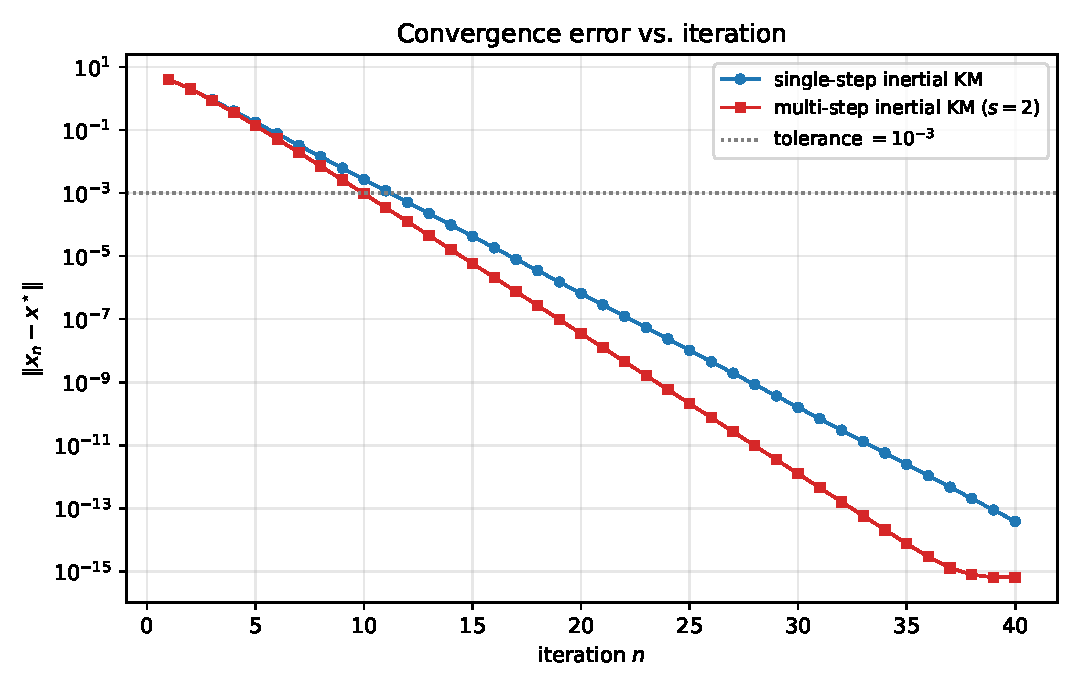
\includegraphics[width=0.47\textwidth]{fig_convergence_error.pdf}

\small Left: trajectories in $\R^2$ (single-step vs.\ multi-step). Right:
$\norm{x_n-x^\star}$ vs.\ $n$ on a log scale -- the multi-step curve drops
below the tolerance line earlier than the single-step curve.
\end{frame}

\begin{frame}{A Cautionary Tale: Why $\theta_1,\theta_2$ Can't Be Too Large}
Since $\Fix(T)$ is the \emph{whole} disk $C$ (every interior point is
already fixed by the projection $T$), overshooting matters: if the
extrapolated point $y_n$ ever lands \emph{inside} $C$, then
$T(y_n)=y_n$ exactly, and the update becomes $x_{n+1}=y_n$ with
\textbf{no further contraction}. With $\theta_1=0.15,\theta_2=0.05$
(a larger total inertial weight $0.20$), $y_n$ enters the disk around
$n=7$ and the sequence \emph{freezes} at $(0.5858,0.7811)$ -- a genuine
element of $\Fix(T)$, but \emph{not} $x^\star=(0.6,0.8)$. This is exactly
the failure mode that condition (6.12)/Remark 6.4 warns about: without a
decay mechanism, $\sum a_n\norm{x_n-x_{n-1}}$ can converge to the
\emph{wrong} limit. Smaller, carefully tuned weights ($\theta_1=0.13,
\theta_2=0.01$ above) accelerate convergence \emph{without} triggering
this instability.
\end{frame}

\begin{frame}[fragile]{Python: Multi-step Inertial KM (Section 6.1)}
\begin{lstlisting}
import numpy as np

def T(x):
    """Projection onto the closed unit disk (nonexpansive)."""
    nrm = np.linalg.norm(x)
    return x / nrm if nrm > 1.0 else x.copy()

def multistep_inertial_km(x0, thetas, lam=0.5, n_iter=30):
    """Multi-step inertial KM with S_n = {0,...,s-1}, b_{n,k}=a_{n,k}
    (Remark 6.4 case: z_n = y_n).  thetas = [theta_1,...,theta_s]."""
    s = len(thetas)
    xs = [x0.copy() for _ in range(s + 1)]      # x_{-1}=...=x_{-s}=x0
    for n in range(n_iter):
        yn = xs[-1].copy()
        for k in range(1, s + 1):
            yn = yn + thetas[k - 1] * (xs[-k] - xs[-k - 1])
        x_next = (1 - lam) * yn + lam * T(yn)
        xs.append(x_next)
    return np.array(xs[s:])                     # drop warm-up copies

x0 = np.array([3.0, 4.0])
traj = multistep_inertial_km(x0, thetas=[0.13, 0.01])
print(traj[9])   # -> (0.600566, 0.800754), already within 1e-3 of (0.6,0.8)
\end{lstlisting}
\end{frame}

%==============================================================
\section{6.2 Parameters Independent of the Iterates}
%==============================================================

\begin{frame}{6.2 Intuition}
\textbf{The problem to solve.} The online rule (6.11) is safe but costly:
recomputing $a_{n,k},b_{n,k}$ at every step, for potentially all $k\in
\{0,\dots,n-1\}$, means the bookkeeping grows with $n$. \textbf{Can we
pick the weights once, in closed form, and never look at $\{x_n\}$
again?} This section gives \emph{two} such pre-scheduled families:
(A) weighted averages of \emph{all} past iterates with hand-picked
weight arrays $\{\mu_{n,k}\},\{\nu_{n,k}\}$, and (B) a \emph{recursive}
exponential-memory variant that can be updated in $O(1)$ time per step.
Both converge \emph{unconditionally} -- no summability condition on
$\{x_n\}$ is required at all.
\end{frame}

\begin{frame}{(A) General KM on the Affine Hull of Orbits}
\begin{block}{Definition (6.13)}
Let $\lambda\in(0,1)$ and let $\{\mu_{n,k}\}_{n\in\N,0\le k\le n}$,
$\{\nu_{n,k}\}_{n\in\N,0\le k\le n}$ be two real arrays (satisfying
technical assumptions (B1)--(B4), notably that each row sums to 1). Take
$x_0\in\Hil$ and, for each $n\ge0$,
\[
\left\{
\begin{aligned}
y_n &= \sum_{k=0}^n \mu_{n,k}\,x_k, \\
z_n &= \sum_{k=0}^n \nu_{n,k}\,x_k, \\
x_{n+1} &= (1-\lambda) y_n + \lambda\, T(z_n).
\end{aligned}
\right.
\]
\end{block}
\textbf{Symbols.} $y_n,z_n$: weighted averages of \emph{every} past iterate
$x_0,\dots,x_n$, using weight rows $\{\mu_{n,k}\}_k$ and $\{\nu_{n,k}\}_k$
that are fixed once, before the algorithm runs, as functions of $(n,k)$
only. Because the weights never reference $\norm{x_i-x_j}$, this scheme
is unconditional by construction.
\end{frame}

\begin{frame}[allowframebreaks]{(A): Reduction to Multi-step Inertial Form}

Telescoping the sum for $y_n$ using $\sum_{k=0}^n\mu_{n,k}=1$ (assumption
(B2)) shows (6.13) is a special case of the general multi-step scheme
(6.5):
\[
y_n = x_n + (\mu_{n,n}-1)(x_n-x_{n-1}) + (\mu_{n,n}+\mu_{n,n-1}-1)(x_{n-1}-x_{n-2})
+\cdots
\]
i.e.\ with $S_n=\{0,\dots,n-1\}$ and
$a_{n,k}=\sum_{j=n-k}^n\mu_{n,j}-1$ (similarly $b_{n,k}$ from $\nu$).

\textbf{Two useful special cases.}
\begin{block}{(6.16): only $y_n$ is averaged}
$\nu_{n,n}=1,\ \nu_{n,k}=0\ (k<n)$, so $z_n=x_n$:
\[
y_n=\sum_{k=0}^n\mu_{n,k}x_k, \qquad x_{n+1}=(1-\lambda)y_n+\lambda T(x_n).
\]
\end{block}
\begin{block}{(6.17): only $z_n$ is averaged}
$\mu_{n,n}=1,\ \mu_{n,k}=0\ (k<n)$, so $y_n=x_n$:
\[
z_n=\sum_{k=0}^n\nu_{n,k}x_k, \qquad x_{n+1}=(1-\lambda)x_n+\lambda T(z_n).
\]
\end{block}
And if $\nu_{n,k}=\mu_{n,k}$ for all $n,k$, (6.13) reduces to the earlier
(single-array) general inertial KM iteration of Chapter 3.

\end{frame}

\begin{frame}{Example 6.1: $(p,q)$-step Inertial KM}
\textbf{Idea.} Instead of averaging over \emph{all} of $x_0,\dots,x_n$,
only average over the last $p$ (for $y_n$) or last $q$ (for $z_n$)
iterates, using \emph{fixed} weights $\{\mu_i\}_{i=0}^p$, $\{\nu_j\}_{j=0}^q$
with $\sum_i\mu_i=\sum_j\nu_j=1$:
\[
\mu_{n,k}=
\begin{cases}
0, & 0\le k< n-p,\\
\mu_{n-k}, & n-p\le k\le n,
\end{cases}
\qquad\text{(similarly for $\nu_{n,k}$ with $q$).}
\]
This is called the \textbf{$(p,q)$-step inertial KM iteration}: $y_n$
looks back $p$ steps, $z_n$ looks back $q$ steps, with hand-chosen
constant weights. By Corollary 6.1 (below), whenever $T$ is nonexpansive
with $\Fix(T)\ne\emptyset$, the $(p,q)$-MiKM sequence converges weakly to a
point of $\Fix(T)$ -- \emph{unconditionally}, i.e.\ this is precisely a
rigorous version of the ``$s$-step method,'' now with a convergence
guarantee that Ortega--Rheinboldt's original proposal lacked.
\end{frame}

\begin{frame}{Example 6.2: Exponential Memory Weights}
\textbf{Idea.} Instead of a hard window of size $p$, let the influence of
older iterates decay \emph{geometrically}. Fix $\mu,\nu\in(0,1)$:
\[
\mu_{n,k}=
\begin{cases}
\mu^{n}, & k=0,\\
(1-\mu)\mu^{\,n-k}, & 1\le k\le n,
\end{cases}
\qquad
\nu_{n,k}=
\begin{cases}
\nu^{n}, & k=0,\\
(1-\nu)\nu^{\,n-k}, & 1\le k\le n.
\end{cases}
\]
\textbf{Reading it.} Writing lag $=n-k$ (how far back), the weight on a
term $x_k$ is $(1-\mu)\mu^{\,\text{lag}}$: the most recent iterate gets
weight $\approx(1-\mu)$, and each step further back is discounted by
another factor of $\mu$ -- an \emph{exponential moving average} (EMA).
This is a bona-fide element of the family (6.13): $\{\mu_{n,k}\}$
and $\{\nu_{n,k}\}$ satisfy the needed structural assumptions (A1)--(A3),
(A5), so by Corollary 6.1 the scheme converges. (Whether the
\emph{combined} array $(1-\lambda)\mu_{n,k}+\lambda\nu_{n,k}$ also
satisfies them for every $\lambda\in(0,1)$ -- needed for the sharper
Theorem 6.4 -- is, interestingly, still \textbf{open}.)
\end{frame}

\begin{frame}{Figure: The Fixed Exponential Weight Schedule}
\centering
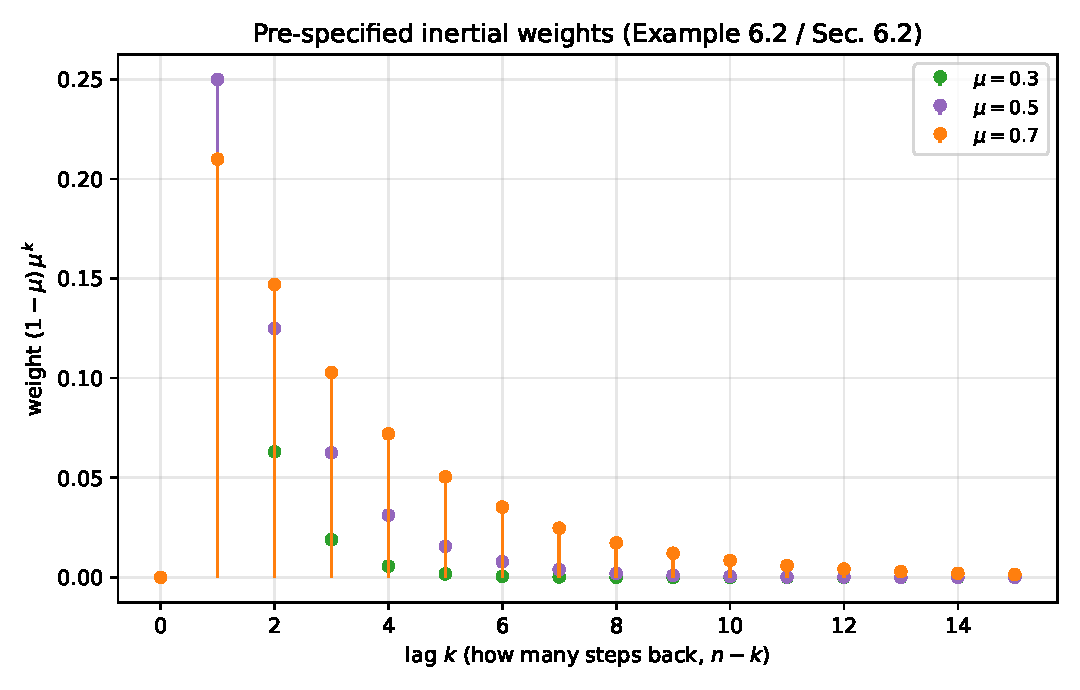
\includegraphics[width=0.62\textwidth]{fig_fixed_weights.pdf}

\small The weight $(1-\mu)\mu^{k}$ assigned to the iterate $k$ steps back,
for three choices of the decay parameter $\mu$. Every one of these curves
is known completely \emph{before} the algorithm is run -- it is a fixed
function of the lag $k$ and does not reference $\{x_n\}$ at all.
\end{frame}

\begin{frame}[allowframebreaks]{Corollary 6.1 and Theorem 6.4}

\begin{block}{Theorem 6.4 (general, weighted)}
Under structural assumptions (B1)--(B4) on $\mu,\nu$, and on
$(1-\lambda)\mu_{n,k}+\lambda\nu_{n,k}$ for every $\lambda\in(0,1)$, plus a
technical summability condition (6.18) involving an auxiliary sequence
$\{\chi_n\}$, the sequence $\{x_n\}$ from (6.13) converges weakly to a
point of $\Fix(T)$.
\end{block}
Condition (6.18) is hard to check directly (it still mixes $\{x_n\}$ into
the picture). \textbf{Good news:} if the arrays are \emph{nonnegative},
this condition can be discharged automatically.

\begin{block}{Corollary 6.1 -- the clean, unconditional statement}
Let $T:\Hil\to\Hil$ be nonexpansive with $\Fix(T)\ne\emptyset$. If
$\{\mu_{n,k}\},\{\nu_{n,k}\}$ are \emph{nonnegative} sequences such that
$\{\mu_{n,k}\}$, $\{\nu_{n,k}\}$, and $\{(1-\lambda)\mu_{n,k}+\lambda\nu_{n,k}\}$
(for all $\lambda\in(0,1)$) satisfy (A1)--(A3) and (A5), then $\{x_n\}$
generated by (6.13) converges weakly to a point of $\Fix(T)$.
\end{block}

This is the payoff: Examples 6.1 and 6.2 both supply nonnegative arrays
satisfying (A1)--(A3),(A5) (Example 6.1 via a known construction, Example
6.2 via [46, Example 2.5]), so \emph{both} the $(p,q)$-step scheme and the
exponential-memory scheme converge weakly to a point of $\Fix(T)$ -- with
\textbf{zero} bookkeeping tied to the run.

\end{frame}

\begin{frame}{(B) The Modified KM Iteration -- A Recursive EMA}
\textbf{Motivation.} Example 6.2's weights are exact, but computing $y_n$
from scratch each time still means summing over all of $x_0,\dots,x_n$ --
an $O(n)$ cost per step. Can the \emph{same} exponential-memory idea be
computed in $O(1)$ time? Yes: keep running EMAs $y_n,z_n$ and update them
recursively.
\begin{block}{Definition (6.19)}
For $x_0,y_0,z_0\in\Hil$, $\lambda\in(0,1)$, $\alpha,\beta\in[0,1]$, and
$n\ge1$:
\[
\left\{
\begin{aligned}
y_{n+1} &= (1-\alpha)x_n + \alpha y_n, \\
z_{n+1} &= (1-\beta)x_n + \beta z_n, \\
x_{n+1} &= (1-\lambda)y_{n+1} + \lambda\, T(z_{n+1}).
\end{aligned}
\right.
\]
\end{block}
\textbf{Symbols.} $\alpha,\beta$: fixed memory-decay constants (bigger
$\Rightarrow$ longer memory); $y_{n+1},z_{n+1}$: the updated EMAs -- each
is just a convex combination of the newest iterate and the previous EMA.
\end{frame}

\begin{frame}{(B): Unrolling the Recursion}
Unrolling $y_{n+1}=(1-\alpha)x_n+\alpha y_n$ (with $y_0=x_0$) gives exactly
\[
y_{n+1}=\sum_{k=1}^n (1-\alpha)\alpha^{n-k}x_k + \alpha^n x_0,
\]
i.e.\ (6.19) with $y_0=z_0=x_0$ is the \emph{same} weighted average as
Example 6.2 (with $\mu=\alpha,\nu=\beta$) -- just computed by carrying one
running vector forward instead of re-summing every time.

\begin{block}{Key practical point -- Remark 6.9}
Computing $x_{n+1}$ in (6.19) only ever needs $x_n,y_n,z_n$ -- it does
\emph{not} need to keep $x_0,x_1,\dots,x_{n-1}$ in memory at all. This is
genuinely cheaper than evaluating the weighted sums of (6.13)/Example 6.2
directly, which do need the full history.
\end{block}
Special cases: $\beta=0$ gives (6.22) (only $y$ is smoothed); $\alpha=0$
smooths only $z$; $\beta=\alpha$ smooths $y$ and $z$ identically; $\alpha=
\beta=0$ recovers the plain KM iteration.
\end{frame}

\begin{frame}{(B): Convergence and Rate -- Theorems 6.5, 6.6}
\begin{block}{Theorem 6.5 -- unconditional convergence}
If $T:\Hil\to\Hil$ is nonexpansive with $\Fix(T)\ne\emptyset$, then
$\{x_n\}$ generated by (6.19) converges weakly to a point of $\Fix(T)$ --
\textbf{for any} fixed $\alpha,\beta\in[0,1]$, $\lambda\in(0,1)$. No
summability condition on $\{x_n\}$ is needed.
\end{block}
\begin{block}{Theorem 6.6 -- running-average complexity bound}
\[
\frac1n\sum_{k=0}^n \norm{x_k-T(x_k)}^2 \le \frac3n\Big(\frac{C}{\tau}+\norm{y_0-T(z_0)}^2\Big), \tag{6.23}
\]
where $\tau=\min\{\lambda(1-\lambda),(1-\lambda)\alpha,\lambda\beta\}$ and
$C=\inf_{x\in\Fix(T)}\{\norm{x_0-x}^2+\tfrac{(1-\lambda)\alpha}{1-\alpha}\norm{y_0-x}^2+\tfrac{\lambda\beta}{1-\beta}\norm{z_0-x}^2\}$.
\end{block}
\textbf{Reading it.} The average residual $\norm{x_k-T(x_k)}^2$ shrinks like
$O(1/n)$, with a constant $C/\tau$ that grows if $\alpha,\beta\to1$
(longer memory, larger constant) or $\lambda\to0,1$ (degenerate KM step).
\end{frame}

\begin{frame}[fragile]{Python: Recursive $O(1)$ Inertial Update (Section 6.2)}
\begin{lstlisting}
import numpy as np

def modified_km_step(x_n, y_n, z_n, alpha, beta, lam, T):
    """One step of the modified KM iteration (6.19): O(1) update,
    parameters alpha, beta, lam are FIXED in advance -- no dependence
    on the run-time sequence {x_n} is needed."""
    y_next = (1 - alpha) * x_n + alpha * y_n
    z_next = (1 - beta) * x_n + beta * z_n
    x_next = (1 - lam) * y_next + lam * T(z_next)
    return x_next, y_next, z_next

def run_modified_km(x0, alpha, beta, lam, T, n_iter=40):
    x_n, y_n, z_n = x0.copy(), x0.copy(), x0.copy()
    hist = [x_n.copy()]
    for _ in range(n_iter):
        x_n, y_n, z_n = modified_km_step(x_n, y_n, z_n, alpha, beta, lam, T)
        hist.append(x_n.copy())
    return np.array(hist)

# alpha, beta play the role of mu, nu in the Example 6.2 weight schedule
traj = run_modified_km(np.array([3.0, 4.0]), alpha=0.5, beta=0.5, lam=0.5,
                        T=lambda x: x / max(np.linalg.norm(x), 1.0))
\end{lstlisting}
\end{frame}

%==============================================================
\section{6.3 Some Applications}
%==============================================================

\begin{frame}{6.3 Intuition}
Every operator-splitting method for $\zer(A+B)$ or a monotone inclusion
that is built out of a nonexpansive map $T$ can be ``inertialized'' by the
same recipe: replace the input to $T$ (and to the resolvent $J_{\gamma A}$
feeding it) with an inertially extrapolated point $y_n$ or $z_n$ built from
$\sum_{k\in S_n}a_{n,k}(x_{n-k}-x_{n-k-1})$, exactly as in (6.5). This
section walks through five such constructions -- forward-backward,
backward-forward, primal-dual, Douglas-Rachford, and Davis-Yin splitting
-- each now with multi-step memory.
\end{frame}

\begin{frame}{(A) Multi-step Inertial Forward-Backward Splitting}
\textbf{Problem.} Find $\zer(A+B)$: e.g.\ minimize $f(x)+g(x)$ where
$A=\partial f$ is the subdifferential of a nonsmooth convex regularizer
(such as $f(x)=\mu\norm{x}_1$, giving LASSO-type sparsity) and
$B=\nabla g$ is the gradient of a smooth, $\beta$-cocoercive loss (such as
$g(x)=\tfrac12\norm{Mx-b}^2$). Then $J_{\gamma A}=\operatorname{prox}_{\gamma f}$.

\begin{block}{Definition (6.24)}
Let $\gamma\in(0,2\beta)$, $\{\lambda_n\}\subset[0,\tfrac{4\beta-\gamma}{2\beta}]$
with $\sum_n\lambda_n(\tfrac{4\beta-\gamma}{2\beta}-\lambda_n)=\infty$:
\[
\left\{
\begin{aligned}
y_n &= x_n + \sum_{k\in S_n} a_{n,k}(x_{n-k}-x_{n-k-1}), \\
z_n &= x_n + \sum_{k\in S_n} b_{n,k}(x_{n-k}-x_{n-k-1}), \\
x_{n+1} &= (1-\lambda_n) y_n + \lambda_n\, J_{\gamma A}(\Id-\gamma B)z_n.
\end{aligned}
\right.
\]
\end{block}
\textbf{Theorem 6.7.} Under condition (6.25) (the (6.9)-type summability
condition), $\{x_n\}$ weakly converges to a point of $\zer(A+B)$.
\end{frame}

\begin{frame}{(B) Multi-step Inertial Backward-Forward Splitting}
\textbf{Problem.} Same $\zer(A+B)$ target, but resolve $A$ \emph{first},
then take a forward (gradient) step in $B$ -- useful when the resolvent of
$A$ is cheap to invert but you would rather not compose it with $B$
directly.
\begin{block}{Definition (6.26)}
\[
\left\{
\begin{aligned}
u_n &= x_n + \sum_{k\in S_n} a_{n,k}(x_{n-k}-x_{n-k-1}), \\
v_n &= x_n + \sum_{k\in S_n} b_{n,k}(x_{n-k}-x_{n-k-1}), \\
y_n &= J_{\gamma A}(v_n), \qquad z_n = y_n - \gamma B y_n, \\
x_{n+1} &= u_n + \lambda_n(z_n-u_n).
\end{aligned}
\right.
\]
\end{block}
\textbf{Theorem 6.8.} With $\delta=\min\{1,\beta/\gamma\}+\tfrac12$, if
$\{\lambda_n\}\subset[0,\delta]$ satisfies $\sum_n\lambda_n(\delta-\lambda_n)=\infty$
and the (6.9)-type condition holds, $\{x_n\}$ (equivalently $\{y_n\}$)
weakly converges to a point of $\zer(A+B)$.
\end{frame}

\begin{frame}{(C) Multi-step Inertial Primal-Dual Splitting}
\textbf{Problem.} A saddle-point / monotone-inclusion system coupling a
primal variable $x$ and a dual variable $v$ through a bounded linear
operator $L:\Hil\to\Gil$ -- e.g.\ TV-regularized imaging or constrained
optimization with $Lx$ appearing inside a nonsmooth penalty. Here $A,C$ are
maximally monotone, $B$ is $\beta_B$-cocoercive, $D$ is $\beta_D$-strongly
monotone, and $\gamma_A,\gamma_C$ satisfy
\[
2\min\{\beta_B,\beta_D\}\min\Big\{\frac1{\gamma_A},\frac1{\gamma_C}\Big\}
\Big(1-\sqrt{\gamma_A\gamma_C\norm{L}^2}\Big) > 1. \tag{6.27}
\]
\begin{block}{Definition (6.28) -- iteration}
\[
\left\{
\begin{aligned}
y_n &= x_n+\!\!\sum_{k\in S_n}\!\! a_{n,k}(x_{n-k}-x_{n-k-1}), \quad
u_n = x_n+\!\!\sum_{k\in S_n}\!\! b_{n,k}(v_{n-k}-v_{n-k-1}), \\
x_{n+1} &= J_{\gamma_A A}(y_n-\alpha B(y_n)-\gamma_A L^\ast u_n), \qquad
\bar x_{n+1} = 2x_{n+1}-y_n, \\
v_{n+1} &= J_{\gamma_C C^{-1}}\big(u_n-\gamma_C D^{-1}(u_n)+\gamma_C L\bar x_{n+1}\big).
\end{aligned}
\right.
\]
\end{block}
\textbf{Theorem 6.9.} Under (6.27) and (6.9)-type conditions on $a_{n,k}$
(applied to the $x$-sequence) and $b_{n,k}$ (applied to the $v$-sequence),
$\{x_n\}$ and $\{v_n\}$ weakly converge to primal/dual solutions.
\end{frame}

\begin{frame}{(D) Multi-step Inertial Douglas-Rachford Splitting}
\textbf{Problem.} $\zer(A_1+A_2)$ via the reflected resolvent operator
$R_{\gamma A_1}R_{\gamma A_2}$, where $R_{\gamma A}=2J_{\gamma A}-\Id$ --
e.g.\ convex feasibility between two sets $C_1,C_2$ (take $A_i=$ normal
cone of $C_i$).
\begin{block}{Definition (6.30)}
With $\gamma>0$, $\{\lambda_n\}\subset[0,2]$, $\sum_n\lambda_n(2-\lambda_n)=\infty$:
\[
\left\{
\begin{aligned}
u_n &= x_n + \sum_{k\in S_n} a_{n,k}(x_{n-k}-x_{n-k-1}), \\
v_n &= x_n + \sum_{k\in S_n} b_{n,k}(x_{n-k}-x_{n-k-1}), \\
x_{n+1} &= \Big(1-\frac{\lambda_n}{2}\Big)u_n + \frac{\lambda_n}{2} R_{\gamma A_1}R_{\gamma A_2}(v_n).
\end{aligned}
\right.
\]
\end{block}
\textbf{Theorem 6.10.} Under the (6.9)-type condition, $\{x_n\}$ converges
weakly to a point of $\Fix(R_{\gamma A_1}R_{\gamma A_2})$ (from which a
zero of $A_1+A_2$ is recovered via $J_{\gamma A_2}$).
\end{frame}

\begin{frame}{(E) Multi-step Inertial Davis-Yin Splitting}
\textbf{Problem.} $\zer(A_1+A_2+B)$, a \emph{three}-operator sum -- e.g.\
minimize $f_1(x)+f_2(x)+g(x)$ with two nonsmooth terms ($A_1=\partial f_1$,
$A_2=\partial f_2$) plus one smooth, cocoercive term ($B=\nabla g$).
\begin{block}{Definition (6.32)}
\[
\left\{
\begin{aligned}
u_n &= x_n + \sum_{k\in S_n} a_{n,k}(x_{n-k}-x_{n-k-1}), \qquad
v_n = x_n + \sum_{k\in S_n} b_{n,k}(x_{n-k}-x_{n-k-1}), \\
y_n &= J_{\gamma A_2}v_n, \\
z_n &= J_{\gamma A_1}(2y_n-v_n-\gamma B y_n), \\
x_{n+1} &= (1-\lambda_n)u_n + \lambda_n(z_n-y_n+v_n).
\end{aligned}
\right.
\]
\end{block}
\textbf{Theorem 6.11.} Under a condition on $\gamma,\lambda_n$ and a
(6.9)-type summability of $a_{n,k}$, the weak limit $x^\ast$ of $\{x_n\}$
satisfies $J_{\gamma A_2}(x^\ast)\in\zer(A_1+A_2+B)$.
\end{frame}

\begin{frame}[fragile]{Python: Multi-step Inertial Forward-Backward (LASSO)}
\begin{lstlisting}
import numpy as np

def soft_threshold(v, t):
    """prox of t*||.||_1 -- the resolvent J_{gamma A} for A = subdiff |.|_1."""
    return np.sign(v) * np.maximum(np.abs(v) - t, 0.0)

def multistep_inertial_fb(M, b, mu, gamma, thetas, n_iter=200):
    """Minimize 0.5*||Mx-b||^2 + mu*||x||_1 via (6.24) with
    b_{n,k}=a_{n,k} (so z_n = y_n), S_n = {0,...,s-1}."""
    d = M.shape[1]
    x = [np.zeros(d) for _ in range(len(thetas) + 1)]   # warm start
    for _ in range(n_iter):
        yn = x[-1].copy()
        for k, th in enumerate(thetas, start=1):
            yn = yn + th * (x[-k] - x[-k - 1])           # multi-step term
        grad = M.T @ (M @ yn - b)                         # B = grad g
        x_next = soft_threshold(yn - gamma * grad, gamma * mu)  # J_{gamma A}
        x.append(x_next)
    return x[len(thetas):]

rng = np.random.default_rng(0)
M = rng.standard_normal((40, 100))
x_true = np.zeros(100); x_true[:5] = rng.standard_normal(5)
b = M @ x_true
sol = multistep_inertial_fb(M, b, mu=0.1, gamma=0.9 / np.linalg.norm(M, 2)**2,
                              thetas=[0.13, 0.01])
\end{lstlisting}
\end{frame}

\begin{frame}{Chapter 6 Summary}
\begin{itemize}
\item \textbf{6.1}: The multi-step inertial KM iteration (6.5) uses a
weighted combination of several lagged displacements
$x_{n-k}-x_{n-k-1}$, $k\in S_n$, generalizing every scheme from Chapter 5.
Weak convergence holds under summability condition (6.9)/(6.10), which in
the single-lag case (Remark 6.4, $b_n=a_n$) reads
$\sum_n a_n\norm{x_n-x_{n-1}}<\infty$ -- a condition that couples the
parameters to the (unknown, in advance) behavior of $\{x_n\}$.
\item \textbf{6.2}: Two ways to \emph{pre-schedule} the inertial weights so
they never reference $\{x_n\}$: (A) weighted averages over a window or with
exponential decay (Examples 6.1-6.2, via (6.13)); (B) a recursive $O(1)$
exponential-moving-average update (6.19) with an \emph{unconditional}
convergence guarantee (Theorem 6.5) and an explicit $O(1/n)$ complexity
bound (Theorem 6.6).
\item \textbf{6.3}: The same multi-step inertial recipe upgrades five
classical operator-splitting methods -- forward-backward, backward-forward,
primal-dual, Douglas-Rachford, Davis-Yin -- each converging to a zero of
the corresponding monotone-operator sum under a matching summability
condition.
\end{itemize}
\end{frame}

\end{document}
